\documentclass[]{article}
\usepackage[left=1in,top=1in,right=1in,bottom=1in]{geometry}
\newcommand*{\authorfont}{\fontfamily{phv}\selectfont}
    \usepackage{lmodern}

\usepackage{amsmath}
  
  \usepackage[T1]{fontenc}
\usepackage[utf8]{inputenc}

\usepackage{abstract}
\renewcommand{\abstractname}{}    % clear the title
\renewcommand{\absnamepos}{empty} % originally center

\renewenvironment{abstract}
{{%
  \setlength{\leftmargin}{0mm}
  \setlength{\rightmargin}{\leftmargin}%
}%
  \relax}
{\endlist}

  
  
  \setcounter{secnumdepth}{0}

\def\tightlist{}

          \usepackage{longtable,booktabs}
  
   \usepackage{graphicx}
  %\graphicspath{ {C:/Users/ryank/Documents/Ryan Sync/Templates/} }
% We will generate all images so they have a width \maxwidth. This means
% that they will get their normal width if they fit onto the page, but
% are scaled down if they would overflow the margins.
\makeatletter
\def\maxwidth{\ifdim\Gin@nat@width>\linewidth\linewidth
  \else\Gin@nat@width\fi}
\makeatother
\let\Oldincludegraphics\includegraphics
\renewcommand{\includegraphics}[1]{\Oldincludegraphics[width=\maxwidth]{#1}}
   
 \makeatletter
\def\@maketitle{%
  \newpage
  
  \null
  \vskip 2.5em
  %\hbox{\vrule height 1pt width 39.14pc}
  %\null
  %\vskip 2em
    %  \begin{center}%
    \let \footnote \thanks
  {\fontsize{18}{20}\selectfont\raggedright  \setlength{\parindent}{0pt} \@title \par}%
}
%\fi
\makeatother 
  
        \title{SPE Curve Comparison between NOAA's COMPASS model and CSS calculations.  }
      
    
    
    \author{\Large Ryan N. Kinzer\vspace{0.05in} \newline\normalsize\emph{Nez Perce Tribe, Department of Fisheries Resources Management}  }
    
    
    \date{}
  
  \usepackage{titlesec}
  
  \titleformat*{\section}{\normalsize\bfseries}
  \titleformat*{\subsection}{\normalsize\itshape}
  \titleformat*{\subsubsection}{\normalsize\itshape}
  \titleformat*{\paragraph}{\normalsize\itshape}
  \titleformat*{\subparagraph}{\normalsize\itshape}
  
  
      
            
    
    \newtheorem{hypothesis}{Hypothesis}
  \usepackage{setspace}
  
  \makeatletter
  \@ifpackageloaded{hyperref}{}{%
    \ifxetex
    \usepackage[setpagesize=false, % page size defined by xetex
                unicode=false, % unicode breaks when used with xetex
                xetex]{hyperref}
    \else
      \usepackage[unicode=true]{hyperref}
    \fi
  }
  \@ifpackageloaded{color}{
    \PassOptionsToPackage{usenames,dvipsnames}{color}
  }{%
    \usepackage[usenames,dvipsnames]{color}
  }
  \makeatother
  \hypersetup{breaklinks=true,
  bookmarks=true,
  pdfauthor={Ryan N. Kinzer (Nez Perce Tribe, Department of Fisheries Resources Management)},
  pdfkeywords = {},  
  pdftitle={SPE Curve Comparison between NOAA's COMPASS model and CSS calculations.},
  colorlinks=true,
  citecolor=blue,
  urlcolor=blue,
  linkcolor=magenta,
  pdfborder={0 0 0}}
  \urlstyle{same}  % don't use monospace font for urls
  
    

  \begin{document}

  % \pagenumbering{arabic}% resets `page` counter to 1 
  %  
    % \maketitle
  
  {% \usefont{T1}{pnc}{m}{n}
  \setlength{\parindent}{0pt}
  %\thispagestyle{plain}
  {\fontsize{18}{20}\selectfont\raggedright 
  \maketitle  % title \par  
  \thispagestyle{empty}
  }
  
  
  {
  \vskip 13.5pt\relax \normalsize\fontsize{11}{12} 
  \textbf{\authorfont Ryan N. Kinzer} \hskip 15pt \emph{\small Nez Perce Tribe, Department of Fisheries Resources Management}   
  
    \hbox{\vrule height .2pt width 39.14pc}
  
  }
  
  }
  
  
    
    
    
  \vskip 6.5pt
  
  \noindent  \begin{figure}
\centering
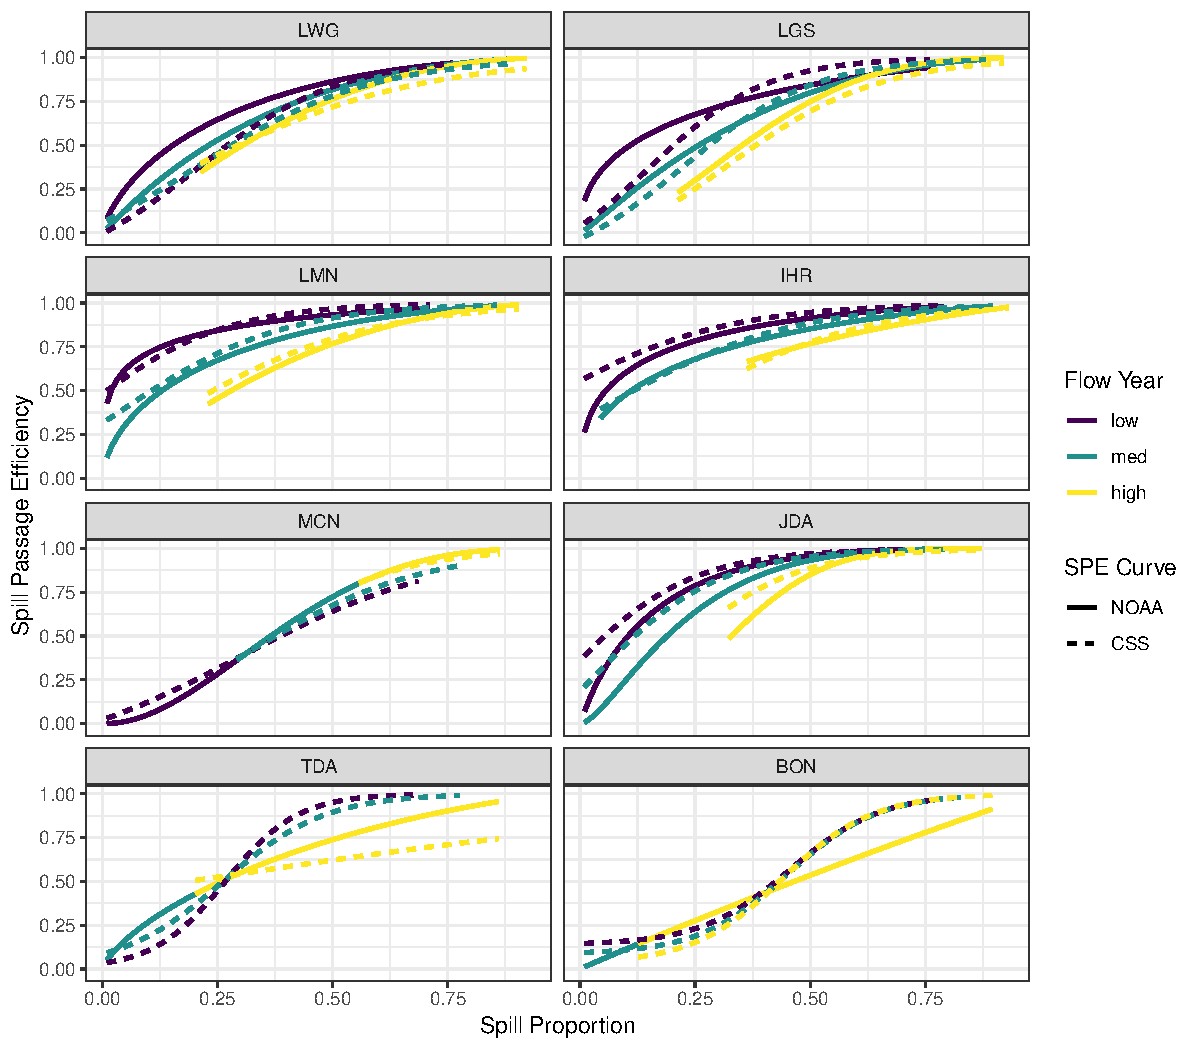
\includegraphics{spe_comparisons_files/figure-latex/unnamed-chunk-4-1.pdf}
\caption{Spill passage efficiency (SPE) curve comparison at low, medium
and high flow volumes; Snake River: 50, 100 and 150 kcfs and Columbia
River: 175, 250, and 400 kcfs.}
\end{figure}

\begin{figure}
\centering
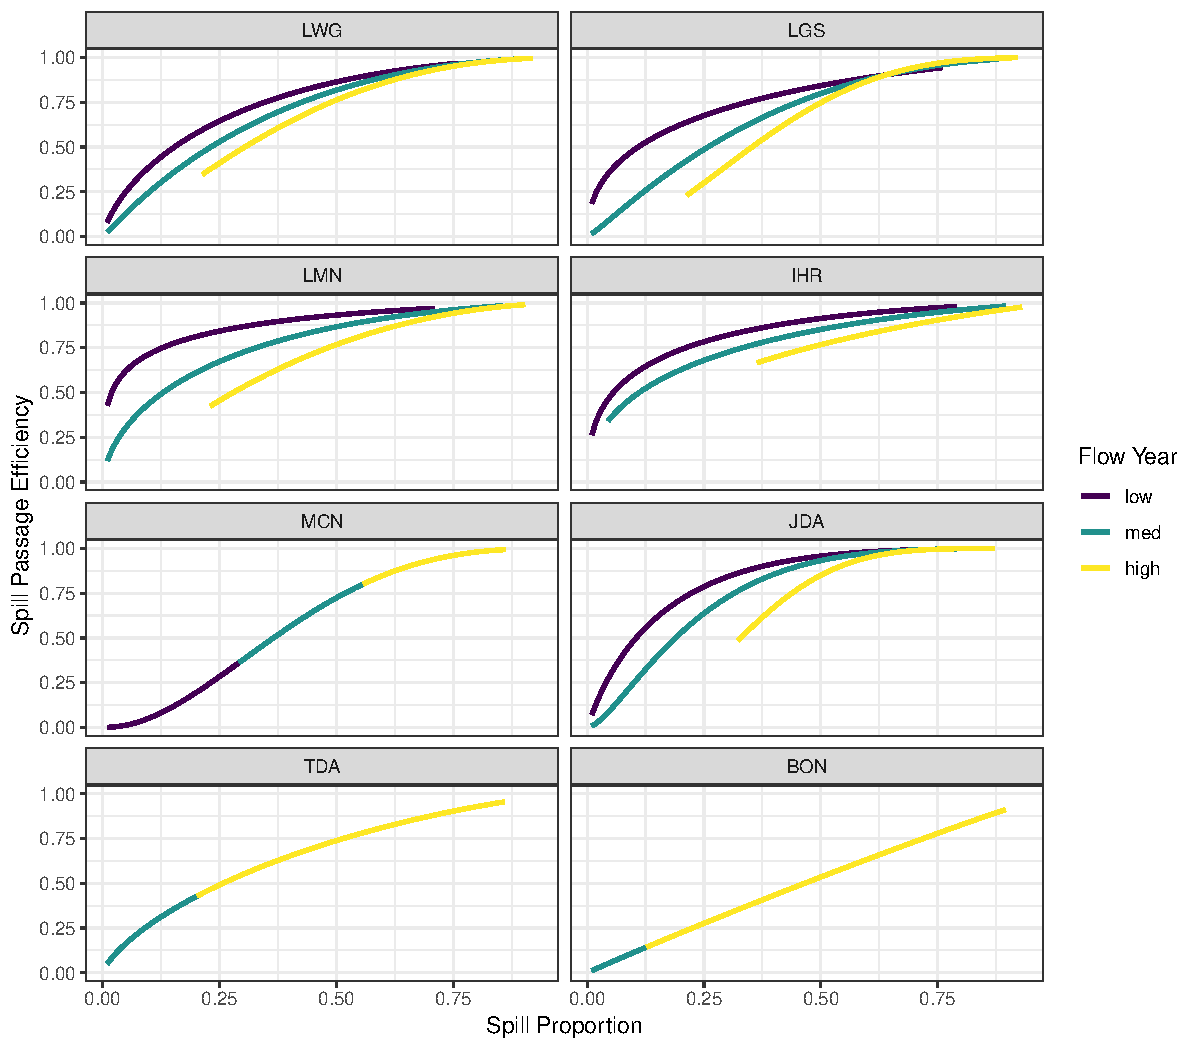
\includegraphics{spe_comparisons_files/figure-latex/unnamed-chunk-5-1.pdf}
\caption{Spill passage efficiency (SPE) curves for NOAA's COMPASS model
at low, medium and high flow volumes; Snake River: 50, 100 and 150 kcfs
and Columbia River: 175, 250, and 400 kcfs.}
\end{figure}

Table 1. Minimum and maximum power house capacity assumption differences
between NOAA's COMPASS model and the values currently used in the Nez
Perce Tribe's PITPH web application tool.

\begin{longtable}[]{@{}lcccc@{}}
\toprule
Project & Minimum - NOAA & Minimum - PITPH & Maximum - NOAA & Maximum -
PITPH\tabularnewline
\midrule
\endhead
LWG & 12.4 & 12.0 & 130 & 118.0\tabularnewline
LGS & 11.6 & 12.0 & 130 & 118.0\tabularnewline
LMN & 11.6 & 14.5 & 130 & 115.5\tabularnewline
IHR & 9.1 & 10.5 & 106 & 95.5\tabularnewline
MCN & 55.0 & 55.0 & 232 & 177.0\tabularnewline
JDA & 55.0 & 51.2 & 322 & 270.8\tabularnewline
TDA & 55.0 & 56.0 & 375 & 319.0\tabularnewline
BON1 & 35.0 & 42.0 & 136 & 349\tabularnewline
BON2 & & & 152 &\tabularnewline
\bottomrule
\end{longtable}
  \newpage
  \singlespacing 
        \end{document}
  Contact GitHub API Training Shop Blog About
  ©